\documentclass{article}
\usepackage[utf8]{inputenc}
\usepackage[english]{babel}
\usepackage{fancyhdr}
\usepackage{graphicx}
\usepackage[ampersand]{easylist}
\usepackage{amssymb}
\ListProperties(Hide=100, Hang=true, Progressive=3ex, Style*=-- ,
Style2*=$\bullet$ ,Style3*=$\circ$ ,Style4*=\tiny$\blacksquare$ )
 
\pagestyle{plain}
\fancyhf{}
\rhead{Version: 0.35}
\chead{Date: 2018-09-14, Doc. Number: PUSS18002}
\lhead{Resp.: PG}
\title{SDP - Software Developement Plan}


\usepackage{lipsum}
\begin{document}

\maketitle
\thispagestyle{fancy}
\tableofcontents
\newpage

\section*{Document history}
 \begin{tabular}{||c c c c||} 
 \hline
 Version & Date & Resp & Description \\ [0.5ex] 
 \hline\hline
 0.3 & 2018-09-14 & PG & Baseline \\ 

 \hline
 

\end{tabular}

\section{Project Organization}
%SDP ska även innehålla en beskrivning av projektorganisationen, där det ska vara tydligt vilka ansvarsområden som finns och vem som har ansvar för vad. Beskriv t ex vem som är projektledare, vem som är med i systemgruppen, vem som är med i testgruppen, vem som är med i de olika utvecklingsgrupperna etc. Beskriv även vilka externa intressenter det finns till projektet.

The project requires a total of 16 people. The current grouping is

\begin{easylist}[itemize]
& PG(2)
&& Assar Pettersson
&& Erik Gralén
& SG(3+1)
&& Jascha Thiel(Leader)
&& Simon Hyttfors
&& Viktor Claesson
&& Daniel Karlsson
& TG (3+1)
&& Jesper Berg(Leader)
&& Jesper Grahm
&& Axel Peterson
&& Tuan Nam Vuong
& UG(3*2)
&& Front-end
&&& Jan Zubac
&&& Filip Karabeleski
&& Back-end
&&& Alexander Pålsson
&&& Sani Mesic
&& Algorithms
&&& Isabella Gagner
&&& Felicia Carlsson
\end{easylist}
\subsection{Project Leaders (PG)}
The project leaders are responsible for bringing the desired product to the client. They need to ensure that the other members of the group are doing the required work by distributing the technical tasks and giving each group member a role(SG, TG or UG). The PG is responsible for creating a proper time schedule in consultation with the other groups and ensure that this schedule is followed throughout the project. 

The project leaders are responsible for identifying and creating a list of the necessary configuration units needed for the project, as well as writing/contributing to some of these such as the SDP, SSD and PR. The configuration units need to be accessible at a (online) document library that the PG also is responsible for managing. They are required to have good contact with the client and the other team members by attending and setting up meetings at least once a week.

The PG has to make sure that each document has an informal and formal examination and distribute the examination work among the group members. They are also active in the Change Control Managemen(CCM).

They have to time report everything they do. The PG is also responsible for completing the final report with metrics and comments from the whole project group. 
\subsection{System Architects (SG)}
The system architect group has the responsibility for the technical aspect in the project. They have a leader who is responsible for reporting in to the PG, and for distributing the work among the members of the SG group. The group leader also has to make sure that the Software Requirement Specification(SRS) is consistent with the Software Verification and Validation Specification(SVVS).

The SG is required to communicate with all the other groups, to ensure that the developer group(UG) and testing group(TG) are working on the same page as well as delegating work tasks to the UG. They are also responsible for configuration management of the work library. The SG are responsible for the compilation of the SRS, STLDD and the SDDD. They are also part of the CCM. 

The SG has to time report everything they do,individually. They are required to participate at formal and informal reviews. During a review they may participate as author of the document or as a reviewer of the document. They may only be a reviewer during informal reviews. They also have to write their conclusions and comments to the Project Final Report(PFR) with their individual experiences.
\subsection{Test Group (TG)}
The test group responsibility is to ensure that everything in the development is properly tested. They have a group leader whose responsibility is to ensure good division of labor, maintain contact with SG and PG, and report all discovered errors to SG.

The group is responsible for creating the SVVS,SVVI and SVVR, as well as to ensure that the SVVS and SRS are consistent. They are also required to participate and help when the UG has to produce automatic unit tests. The TG has the responsibility of the system construction and to ensure that the system is regression tested. 

The TG has to time report everything they do, individually. Participate as author and/or examiner in document examinations(both informal and formal). They also has to compile their conclusions and comments to the end report coherent with what they have done.  

\subsection{Developers (UG)}
The developers are responsible for the development of the functionality to the project. They are divided into three sub-groups: Back-end, front-end and algorithms. Each sub-group is responsible for the functionality coherent to that sub-group. The functionality is required to follow and be consistent to requirements given from the SRS. They are required to produce sub-chapters to the SRS,STLDD and SDDD.

The UG have to time report everything they do,individually. They are required to participate at formal and informal reviews. During a review they may participate as author of the document or as a reviewer of the document. They may only be a reviewer during informal reviews. They also have to write their conclusions and comments to the Project Final Report(PFR) with their individual experiences.

\subsection{Change Control Management(CCM)}
The Change Control Management consists of the PG and SG. The purpose of this group is configuration management of all the produced documents. The SG has main responsibility for this and the PG participates with making decisions of change operations that requires resource and time-planning. 

\subsection{External Members}
The organization has several external members. The external members are the section manager, the client, a formal examiner and some technical experts. The section manager, responsible to help the project groups if they are in dire need with anything non-technical. The client is the mission-giver to the group and also the recipient of the final product. The formal reviewer examiner is conducting the formal reviews and controls that the development plan is followed. 

There are three technical experts that the group can consult if their respective expertise is needed. A requirements expert, a test expert and a design expert.

The external members are:
\begin{itemize}  
\item Section manager - Anders Bruce - Anders.Bruce@cs.lth.se
\item Requirements expert - Johan Linåker - Johan.Linaker@cs.lth.se
\item Design expert - Sergio Rico - sergio.rico@cs.lth.se
\item Test expert - Anders Bruce - Anders.Bruce@cs.lth.se
\end{itemize}

\subsection{Contact}
Below is a contact list of all group members
\begin{itemize}  
\item Assar Pettersson - mat13ape@student.lu.se
\item Erik Gralén - dat15egr@student.lu.se
\item Jascha Thiel - dat14jth@student.lu.se
\item Simon Hyttfors - simon.hyttfors.214@student.lu.se
\item Viktor Claesson - viktor.claesson.923@student.lu.se
\item Daniel Karlsson - daniel.karlsson.536@student.lu.se
\item Jesper Berg - jesper.berg.850@student.lu.se
\item Jesper Grahm - jesper.grahm.770@student.lu.se
\item Axel Peterson - axel.peterson.282@student.lu.se
\item Tuan Nam Vuong - tuan.n.vuong@gmail.com
\item Jan Zubac - jan.zubac.424@student.lu.se
\item Filip Karabeleski - filip.karabeleski.643@student.lu.se
\item Alexander Pålsson - alexander.palsson.143@student.lu.se
\item Sani Mesic - sani.mesic.348@student.lu.se
\item Isabella Gagner - tfy15iga@student.lu.se
\item Felicia Carlsson - felicia.carlsson.347@student.lu.se
\end{itemize}



\section{Time Plan}
%I tidplanen ska det finnas en detaljerad nedbrytning av det arbete som ska ske i aktiviteter. Det ska också finnas skattningar av arbetstid (dvs “effort”), ledtid och datum för när aktiviteter ska vara färdiga. Det betyder att man ska kunna utläsa minst följande:
The project is divided into four phases. Each phase has a set of deliverables that has to be sent in within the given deadline. Before the deadline, the deliverables are to be reviewed internally within the group. After the internal review the deliverables shall undergo a formal review by a reviewer chosen by the section. A phase is finished when the reviewer approves the deliverables. 

The phases are:
\begin{enumerate}  
\item  \textit{Specification} - During this phase three documents are produced. The first document is the Softare Developement Plan(SDP) which contains detailed information about the project and a time plan. Also, during this phase the requirements of the product are specified into a document called the Software Requirements Specification(SRS), this is the second document. The final document is the Software Verification and Validation Specification(SVVS), this document contains details about how the testing of the development will be conducted, quality assurance and a validation specification. The deliverables of this phase is the SDP, SRS and SVVS.
\item \textit{High Level Design and Test Instructions} - In this phase the high level architecture of the system will be decided along with test instructions based on the cases from the SVVS. The high level design about the different components and how they communicate will be documented to the Software Top Level Design Document(STLDD) and the test instructions will be documented to the Software Verification and Validation Instruction(SVVI). These two documents are the deliverables of this phase.  
\item \textit{Low Level Design} - This phase focuses on the implementation of the high level design. During this phase a document called the Software Detailed Design Document(SDDD) is produced that contains specifications of all system components along with the implemented code. The SDDD is the single deliverable of this phase.
 \item \textit{Integration and system testing} - In this phase the system components are integrated to a single system. The system also has to be verified by the function and system tests. All verification and validations during the project are to be documented to the Software Verification and Validation Report (SVVR). If the system quality is acceptable it is to be delivered to the client and the delivery is documented to a System Specification Document(SSD). The project along with the group members individual experiences is documented to the Project Final Report(PFR).  
\end{enumerate}

\subsection{Effort and time estimations}
%1. Skattad tidsåtgång för varje fas (hur fördelas arbetsinsatsen över projektets faser?).
%2. Skattad start- och slutdatum för varje fas (när blir olika delar klara?).
%3. Skattad tidsåtgång för varje dokument (vad kostar varje del?).
%4. Skattad start- och slutdatum för varje dokument (när blir olika dokument klara?).

\subsubsection{Phase 1 - Specification}
Phase 1 begins at 06/09, and has a deadline at 16/09. This gives 10 days of work spent on this phase. During this phase the SDP, SRS and SVVS are to be produced. These documents are produced by PG, SG and TG respectively. 

The most important document of this phase is the SRS and for that reason SG has the most amount of work this phase. The UG group also has to contribute to the SRS but not as much as the SG group. 

Since SVVS has to be coherent with SRS, the SRS should be done before some parts of the SVVS is written. The production of the SDP and SRS should start at the same date as the phase begins. The deadline of all these documents is the same as the phase deadline. 


\subsubsection{Phase 2 - High Level Design and Test Instructions} Phase 2 begins at 17/09 and has its deadline at 27/09. As with phase 1 this gives the group 10 days to complete the STLDD and SVVI.  

During this period the PG and UG do not have much required work. For SG the workload is quite heavy during this period, the STLDD is a crucial document for the next phase and contains much information about the high level design. During this phase the TG are responsible for creating the SVVI.

The prodcution of STLDD should start at the same date as the phase begins, as well should the SVVI for good measurements. The deadline of these documents are a couple days before the phase deadline so there is time for an informal review as well as any corrections from this review.

\subsubsection{Phase 3 - Low Level Design}
This phase begins at 01/10 and has a preliminary deadline at 14/10. During this phase most of the work is done by the UG since they are responsible for the code implementation. SG is responsible for creating the SDDD during this phase.

The production of the SDDD starts when the phase begins. As with phase 2 the document should be done a few days before the deadline to make sure the group has time to do an informal review and any corrections from this review to the SDDD.

\subsubsection{Phase 4 - Integration and System Testing}
The phase begins at 15/10 and has a deadline at 24/10. It possible that this phase may begin earlier and run parallel with the end of phase 3 but it depends on how well phase 3 is going. In this phase PG is responsible for producing the SSD, as TG is for the SVVR. All groups must also contribute to the PFR. 

The production of SVVR may start when the phase begins, as with the SSD. When these documents are done all effort should go to the production of the PFR. The deadline for all documents is the same as the phase deadline.  

\subsection{Time estimation of other activities}
%5. Skattad tidsåtgång för olika aktiviteter och aktivitetstyper i respektive fas (vad lägger man tiden på?). (Möten, granskningar, ändringshantering, rapportering, etc.)
During the project there are other activities such as meetings, reviews and configure management. Each week there will be at least one project meeting for the whole group. This meeting will last approximately 30 minutes. 

After each phase, a formal review meeting will be held. There are at least four formal meetings and each meeting will last approximately 1 hour. If a baseline is unapproved, the reviewer may require an additional formal meeting. Before each formal review an informal review must be held. The group has chosen to do the informal reviews digitally. An informal review may take up to 1 hour or more depending on size and amount of errors on the document being reviewed.

Time will also be spent on configuration management. Configuration management is the process of a change being treated to a document. This is necessary because it enables parallel work between the phases and documents. Configuration management is only done by PG and SG and the amount of time spent on this depends on how well and error-less the development is. 

\subsection{Time estimation: Groups}
%6. Skattad tidsåtgång för varje grupp, uppdelat per vecka (går det in på en 40-timmarsvecka?).
In figure \ref{grouph} is a table of estimated work hours per each group, for each week. 

\begin{figure}[h]
\centering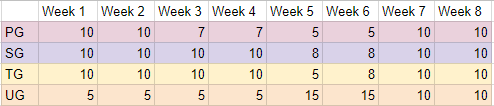
\includegraphics[width=0.8\textwidth]{grupptimmar.PNG}
\caption{\label{grouph} Estimated group time effort}
\end{figure}


\subsection{Estimation uncertainties}
%Ange även i projektplanen vilka metoder ni använt för att göra skattningar av tid och kostnad, samt vilka de största osäkerheterna är med skattningarna.
One of the uncertainties with the time estimations is if a baseline is not approved after the formal review. If the baseline is unapproved, work has to be done to fix this, and the amount of time needed to be spent on this is hard to predict. If much work is needed some deadlines may have to be pushed. 

The amount of hours each group has to work each week is also an uncertainty. The numbers may vary depending on how well or bad the development is going. 

\subsection{Calendar}
%7. En kalenderplan där man kan se vad varje grupp ska göra varje vecka (vem ska göra vad och när?). Detta kan t ex åskådliggöras i ett “Gantt-schema”.
In figure \ref{Calendar} is a preliminary calendar overview of the project.

\begin{figure}[h]
\centering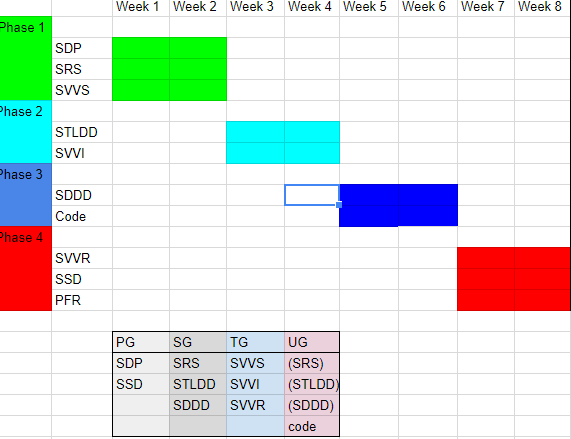
\includegraphics[width=0.8\textwidth]{calendar.PNG}
\caption{\label{Calendar} Time plan overview}
\end{figure}

\section{Project Library and Configurement Management}
All documents and code which are version controlled will be stored on the team's Git server. The master branch will only contain documents and code that have been approved by CCM. 

\section{Tools and Methods}

The following tools and software will be used by team members when working on the project:

\begin{itemize}
    \item Slack for all communication within the group.
    \item Overleaf and LaTeX to write documents.
    \item Github and Git to handle version control of code and documents.
    \item E-puss to handle time reporting, error reporting and status reporting.
\end{itemize}

The following tools will be used to develop the product:
\begin{itemize}
    \item Java, Jetty, and Jersey in back-end implementation.
    \item SQL and H2 to implement database.
    \item HTML, CSS, Javascript and Bootstrap in front-end web client implementation.
    \item Jenkins to automate unit-tests. 
\end{itemize}

\section{Follow-up and Quality Evaluation}
%Det ska finnas en del i projektplanen som beskriver hur uppföljning, t ex av tidplanen, sker under projektet, samt vad som händer om arbetet inte verkar gå enligt plan. Det ska också finnas en beskrivning av de rutiner som finns för kvalitetsutvärdering under projektet.
\subsection{Follow-up}
As the project progresses, the group may start to deviate from the original plan. This can be either voluntary or involuntary changes. It is important to take note of these changes so that they can be handled and evaluated accordingly. As such, all deviations will be discussed in our weekly meetings and/or reported through other means. While everyone in the group must communicate if they notice or predict deviations, the main responsibility of handling and evaluating them lies with the PG. 

Since changes are likely to occur, it is important that the group has a clear guideline to handle them.
\begin{enumerate}  
\item  \textit{Identify} - If any group member notices or predicts problems or changes, this person must inform the rest of the group. This can be done during one of our meetings or through Slack.
\item \textit{Analyze} - PG and key team members analyze potential effects. Additionally, the PG may perform a root cause analysis if it seems appropriate. 
\item \textit{Response} - PG and key team members decides the appropriate response and informs the rest of the group. 
 \item \textit{Evaluate} - PG and key team members evaluate if the response was effective, if this deviation was predictable, and what measures could have been taken to avoid it. 
\end{enumerate}

All of these steps should be recorded and discussed internally. 


\subsection{Quality Evaluation}
During the project, quality evaluations will be done through formal reviews, informal reviews, and testing. Formal reviews will be held during each phase with appropriate team members and external members. Informal reviews will be held before each formal review and when otherwise deemed appropriate by PG. PG will either select a few members to review or select the whole group. This group must then individually read and review the documents and send feedback via Slack. Testing will be in the form of both unit tests (UG) and black-box testing (TG).


\section{Risk Analysis}
%I projektplanen ska även resultatet av en riskanalys för projektet presenteras. Ange hur riskanalys utförts i projektet, samt de viktigaste riskerna som identifierats. rapportera åtminstone följande för varje rapporteras risk: skattad sannolikhet (t ex, låg, medel, hög), skattad effekt (t ex, låg, medel, hög), möjliga indikatorer på att risken förvekligas, samt exempel på lösningar om risken förverkligas.

\textbf{Disengagement}, \textit{low risk, medium impact} - A member becomes disengaged with the project. This can mean not doing the required work, not showing up to meetings or not communicating well. This can be solved by trying to reengage the member, changing roles or redistributing work. 

\textbf{Internal conflicts}, \textit{high risk, low impact} - All conflicts between members will hopefully be handled professionally. If the members can not solve the conflict themselves, other team members can help. If major conflict occur, members should discuss and decided whether to try to solve it internally or externally. 

\textbf{Poor communication}, \textit{medium risk, medium impact} - This may be between groups, in the whole group, internally within a group, or with external members. It this problem arises, more meetings can be arranged to hold discussions. During each meeting, the team should discuss the level of communication. 

\textbf{Poor planning}, \textit{medium risk, medium impact} - Due to inexperience with the project process, there is a risk of certain aspects being overlooked or estimated poorly. Provided resources should therefore be utilized effectively. PG and others should continuously evaluate the progress and plan. 

\textbf{Lack of technical competence}, \textit{low risk, high impact} - Although there will be many new concepts to learn, our team will be able to support each other and take time to learn. In meetings, the team should discuss if there are some things that members should learn beforehand. If required, PG can reassign roles, provide support from other groups, or redesign the plan to be more realistic. The development phase is also expected to include a learning curve. 

\textbf{Poor design}, \textit{low risk, high impact} - The high-level design might need to be redesigned and large amounts of work needs to be redone. Since our project is rather small and built upon a preexisting system, the risk is rather small. To further minimize the risk, all designs should be properly evaluated.

\textbf{Improper reporting}, \textit{medium risk, medium impact} - Members might fail to properly report, for example, changes and time. This might lead to miscommunication or inaccuracies. All members should utilize the course material and PG communicate the importance of it. 

\textbf{Unexpected amount of paperwork}, \textit{high risk, medium impact} - Members might have an unrealistic expectation regarding the amount of paperwork. This can result in slower progress or not following the project process correctly. The group should discuss this early and prepare. 

\bibliographystyle{plain}
\bibliography{refer}
\end{document}
